\documentclass{article}
\usepackage[utf8]{inputenc}
\usepackage{amsmath}
\usepackage{graphicx} 
\usepackage{enumitem}
\usepackage{listings}
\usepackage{float}


\title{Poročilo o projektni nalogi pri predmetu Matematično modeliranje}
\author{Matija Krigl}
\date{May 2024}

\begin{document}

\maketitle

\tableofcontents

\section{Naloga}
    Dana je diskretna verižnica (podatki so mase in dolžine posameznih členkov ter obesišči verižnice).
    
    \begin{enumerate}[label=(\alph*)]
        \item Za vsak posamezen členek verižnice določite njegovo težišče.
        \item Skozi obesišči verižnice in težišče vsakega posameznega členka napeljite interpolacijski polinom \( p \).
        \item Izračunajte dolžino \( l \) polinoma \( p \) med obesiščema.
        \item Določite zvezno verižnico, ki poteka skozi dani obesišči in ima dolžino enako \( l \). Kakšna je razdalja med najnižjo točko polinoma \( p \) (gledano med obesiščema) in najnižjo točko zvezne verižnice?
    \end{enumerate}
    
\section{Diskretna verižnica in iskanje težišč}
    \subsection{Matematično ozadje}
        \textit{Diskretna verižnica} je vrv sestavljena iz gibko vpetih togih členkov, palic. Imenujemo jo \textit{verižnica}, ker ima obliko prosto obešene vrvi.   
    
        Naj bo diskretna verižnica sestavljena iz \(n+1\) členkov dolžin
        \[ L_i, \quad i = 1, 2, \ldots, n+1 \]
        in mas
        \[ M_i, \quad i = 1, 2, \ldots, n+1. \]
        
        Da bi določili težišča posameznih členkov, moramo najprej izračunati koordinate njihovih krajišč:
        \[ (x_i, y_i), \quad i = 0, 1, \ldots, n+1, \]
        kjer sta obeščišči podani kot \((x_0, y_0)\) in \((x_{n+1}, y_{n+1})\).

        \begin{figure}[h!]
        \centering
        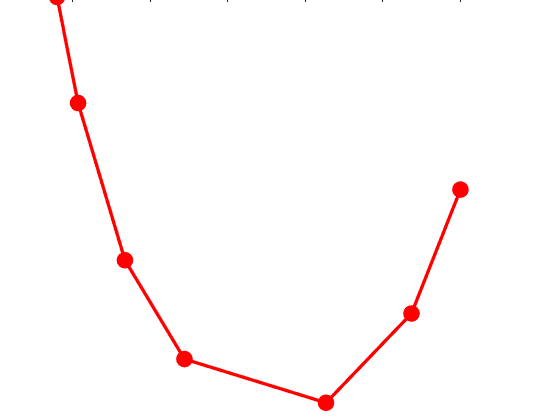
\includegraphics[width=0.5\linewidth]{primerDiskretneVeriznice.png}
        \caption{Primer diskretne verižnice sestavljene iz 6-tih členkov.}
        \label{slika1:diskretna}
        \end{figure}

        Ravnotežne pogoje dosežemo z zahtevo, da je težišče čim nižje, kar je ekvivalentno minimizaciji potencialne energije.
        
        Koordinati težišča palice izračunamo kot srednjo vrednost koordinat obeh koncev palice. Zato moramo poznati koordinate prijemališč ravne palice \(A(x_{i-1}, y_{i-1})\) in \(B(x_i, y_i)\). Vsak par zaporednih točk je enako oddaljen kar ustreza radiju krožnice. 
        Težišče palice \(T_i(\alpha_i, \beta_i)\):

        \[
        \alpha_i = \frac{x_{i-1} + x_i}{2}
        \]
        
        \[
        \beta_i = \frac{y_{i-1} + y_i}{2}
        \]
        
        To lahko zapišemo tudi kot vektor:
        \[
        T_i = \left( \frac{x_{i-1} + x_i}{2}, \frac{y_{i-1} + y_i}{2} \right)
        \]

        Vezani ekstrem prevedemo na neveznega z uvedbo Langrangeovih multiplikatorjev. Ravnotežne enačbe dobimo z odvajanjem nevezanega ekstrema funkcije s parcialnim odvajanjem po \(x_i\), \(y_i\), in \(\lambda_i\). Problem prevedemo na sistem 3n+1 enačb za 3n+1 neznank.

        \begin{align*}
            \xi_i &= x_i - x_{i-1}, \quad i = 1, 2, \ldots, n+1, \\
            \eta_i &= y_i - y_{i-1}, \quad i = 1, 2, \ldots, n+1.
        \end{align*}

         Vpeljemo tudi spremenljivko za delno vsoto \(\mu_i\): 
        \begin{equation*}
        \mu_i = \frac{M_i + M_{i+1}}{2}.
        \end{equation*}



    \subsection*{Funkcija F\_uv - Matlab} 
        Funkcija ima spremenljivko \texttt{w} in vrne vrednost vektorske funkcije za diskretno verižnico.
        
       Izračunamo \texttt{kvoc}:
        
        \begin{equation*}
            \frac{\eta_i}{\xi_i} = v - u \sum_{j=1}^{i-1} \mu_j, \quad i = 1, 2, \ldots, n + 1,
        \end{equation*}
        
        Z uporabo \texttt{kvoc} izračunamo vektorja \(\theta\) in \(\xi\). Ker velja
        \begin{align*}
            U(u, v) &= \sum_{i=1}^{n+1} \xi_i - (x_{n+1} - x_0), \\
            V(u, v) &= \sum_{i=1}^{n+1} \eta_i - (y_{n+1} - y_0),
        \end{align*}
        smo problem prevedli na manjši sistem. \\
        Z uporabo \texttt{fsolve} poiščemo ničle funkcije. Tako izboljšamo začetni približek \texttt{w\_0} določimo neznanki \(v\) in \(u\). 
        
    \subsection*{Funkcija diskrVeriznica - Matlab}
        Ko najdemo \( u \) in \( v \), lahko izračunamo horizontalne (\(\xi_i\)) in vertikalne (\(\eta_i\)) komponente za vsak členek.

        Velja: 
        \begin{equation*}
        \xi_i = \frac{L_i}{\sqrt{1 + \left( v - u \sum_{j=1}^{i-1} \mu_j \right)^2}}, \quad i = 1, 2, \ldots, n + 1,
        \end{equation*}
        in         
        \begin{equation*}
            \eta_i = \xi_i \left( v - u \sum_{j=1}^{i-1} \mu_j \right), \quad i = 1, \ldots, n + 1.
        \end{equation*}
    
        Izračunamo koordinate \(x\) in \(y\). \(\xi\) predstavlja horizontalne razdalje med vozlišči,\(\eta\) pa predstavlja vertikalne razdalje med vozlišči.\texttt{cumsum} izračuna kumulativno vsoto teh razdalj in dobimo končne koordinate \(x\) in \(y\).
        

    \subsection*{Funkcija dolociTezisce - Matlab}
        Funkcija uporablja vektorske operacije za izračun težišč. Koordinate členkov v matriki (\textit{koordinate\_clenkov}). Težišča se izračunajo tako, da vzamemo povprečje vsakega para sosednjih točk.
        \medskip

\section{Interpolacija polinoma}
    \subsection{Matematično ozadje}
        Interpolacija polinomov je metoda, s katero najdemo polinom, ki gre skozi nabor danih točk. Predpostavimo, da imamo \( n \) točk \((x_1, y_1), (x_2, y_2), \ldots, (x_n, y_n)\). Želimo najti polinom \( P(x) \) stopnje \( n-1 \), ki zadošča pogoju:
        \[
        P(x_i) = y_i \quad \text{za vse} \quad i = 1, 2, \ldots, n.
        \]
        V našem primeru so točke \((x_1, y_1), (x_2, y_2), \ldots, (x_n, y_n)\) koordinate dveh obesišč verižnice in težišč vsakega posameznega členka.

        \subsection*{Funkciji \texttt{polyfit} in \texttt{polyval} - Matlab} 
        Funkciji \texttt{polyfit} in \texttt{polyval} omogočata delo s polinomsko interpolacijo in evalvacijo polinomov. Povežimo to s konceptom interpolacije polinomov.
        
        \textbf{Funkcija \texttt{polyfit}} je MATLAB-ova funkcija, ki izračuna koeficiente polinoma, ki najbolje ustreza naboru podatkov v smislu najmanjših kvadratov. Če imamo podatke \((x, y)\), uporaba funkcije \texttt{polyfit} je:
        \[
        p = \texttt{polyfit}(x, y, n)
        \]
        kjer je: \( x \) vektor abscis (x-koordinat) podatkovnih točk; \( y \) je vektor ordinat (y-koordinat) podatkovnih točk; \( n \) stopnja polinoma.
        Funkcija \texttt{polyfit} vrne vektor koeficientov polinoma  
        \( p(x) = p_1 x^n + p_2 x^{n-1} + \ldots + p_{n+1} \). 
        \\
        
        \vspace{0.1cm}
        \textbf{Funkcija \texttt{polyval}} je MATLAB-ova funkcija, ki vrednoti polinom z danimi koeficienti pri določenih vrednostih \( x \). Če imamo polinom določene koeficiente \( p \), uporaba funkcije \texttt{polyval} je:
        \[
        y = \texttt{polyval}(p, x)
        \]
        kjer je: \( p \) vektor koeficientov polinoma;  \( x \) so točke, pri katerih želimo vrednotiti polinom.

        \begin{figure}[h!]
        \centering
        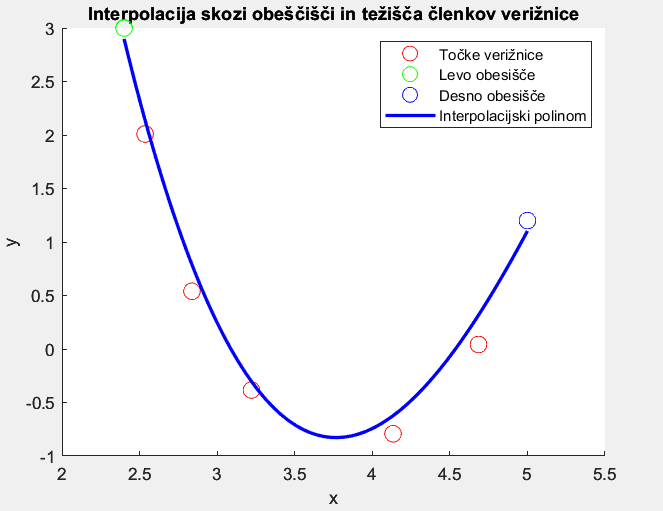
\includegraphics[width=0.8\linewidth]{slikaInterpolPol.png}
        \caption{Primer interpolacije polinoma iz 6-tih členkov.}
        \label{slika2:interpolacija}
        \end{figure}
        \medskip
        
        \section{Izračun dolžine krivulje}
        \subsection{Matematično ozadje}
        Dolžina krivulje, ki jo opisuje polinom med dvema točkama, temelji na formuli za dolžino krivulje v ravnini.

        Dolžina krivulje je enaka vsoti neskončno majhnih segmentov krivulje.
        Majhen segment dolžine krivulje \( ds \) med dvema točkama \( (x, y) \) in \( (x + dx, y + dy) \) je podan z:
        \[
        ds = \sqrt{dx^2 + dy^2}
        \]
        
        Če izrazimo \( dy \) v odvisnosti od \( dx \), dobimo:
        \[
        ds = \sqrt{1 + \left( \frac{dy}{dx} \right)^2} \, dx
        \]
        
        Celotna dolžina krivulje med točkama \( x = a \) in \( x = b \) je torej:
        \[
        l = \int_a^b \sqrt{1 + \left( \frac{dy}{dx} \right)^2} \, dx
        \]

    \section{Razdalja med najnižjema točkama}
        \subsection*{Najnižja točka interpolacijskega polinoma}
        Prvi odvod polinoma \( p \) je polinom \( dp \). Kadar je prvi odvod enak nič, imamo stacionarno točko. Na tej točki je bodisi maksimalen, minimalen ali ima točko prevoja. Polinom predstavljen s svojimi koeficienti nam polyder vrne koeficiente odvoda tega polinoma.

        \begin{equation*}
            dp = \text{polyder}(p)
        \end{equation*}
        
        Iskanje ničel prvega odvoda (stacionarne točke):
        \begin{equation*}
            \text{stacionarne\_tocke} = \text{roots}(dp)
        \end{equation*}
        Funkcija \texttt{roots(dp)} najde ničle polinoma \( dp \) (oz. stacionarne točke polinoma \( p \)).
    
        Relavantne stacionarne točke ležijo znotraj intervala \([a, b]\). Filtriramo stacionarnih točk znotraj intervala \([a, b]\).
    
        Izračunamo še vrednosti polinoma v stacionarnih točkah:
        \begin{equation*}
            \text{vrednosti\_relavantnih} = \text{polyval}(p, \text{relavantne\_stacionarne})
        \end{equation*}
        Funkcija \texttt{polyval(p, relavantne\_stacionarne)} izračuna vrednosti polinoma \( p \) v filtriranih stacionarnih točkah.
    
        Izračun vrednosti polinoma na robovih intervala:
        \begin{equation*}
            \text{rob\_a} = \text{polyval}(p, a)
        \end{equation*}
        \begin{equation*}
            \text{rob\_b} = \text{polyval}(p, b)
        \end{equation*}
    
        Nato izračunamo vse pomembne vrednosti in združimo vrednosti polinoma v vseh relevantnih točkah (stacionarnih točkah in robovih intervala) in njihove koordinate.
        
        \begin{lstlisting}[language=Matlab]
    vrednosti_interp_pol = [vrednosti_relavantnih; rob_a; rob_b];
    tocke_interp_pol = [relavantne_stacionarne; a; b];
        \end{lstlisting}

        Uporabimo funkcijo \texttt{min}, da najdemo najmanjšo vrednost izmed vseh relevantnih vrednosti. \texttt{min\_value} bo najmanjša vrednost, \texttt{min\_index} pa indeks, kjer se ta vrednost pojavi. \texttt{najnizja\_tocka\_pol} bo koordinata \( x \), kjer polinom doseže to najmanjšo vrednost.

        \begin{lstlisting}[language=Matlab]
        [min_value, min_index] = min(vrednosti_interp_pol);
        najnizja_tocka_pol = tocke_interp_pol(min_index);
        \end{lstlisting}
        
        \begin{figure}
            \centering
            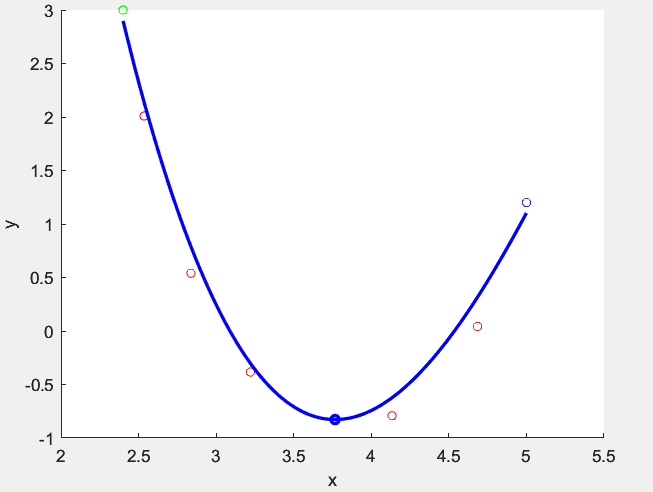
\includegraphics[width=0.8\linewidth]{najnizjaInterpolacijskegaPolinoma.png}
            \caption{Primer interpolacijskega polinoma in njegov minimum}
            \label{fig:enter-label}
        \end{figure}


    \subsection*{Zvezna verižnica}
        Zvezna verižnica opisuje obliko idealne vrvi, ki je obešena med dvema točkama in podvržena samo svoji teži. 
        
        \begin{figure}[h!]
        \centering
        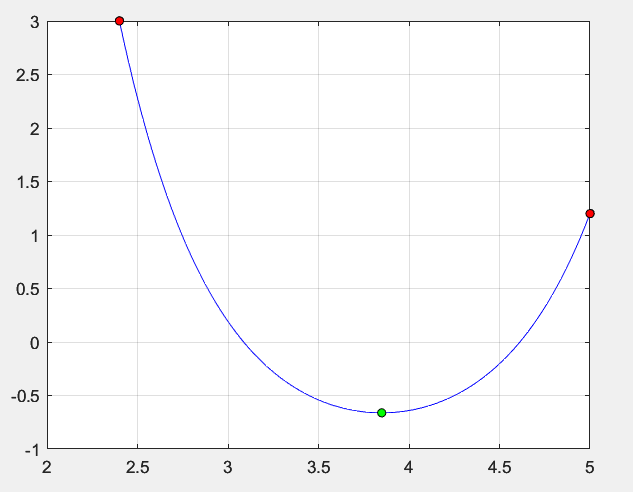
\includegraphics[width=0.8\linewidth]{zveznaVeriznica.png}
        \caption{Primer zvezne verižnice in njen minimum}
        \label{slika3:interpolacija}
        \end{figure}
        \medskip

    Oblika verižnice je podana z enačbo:
        \[
        y = a \cosh\left(\frac{x}{a}\right),
        \]
        kjer je \( \cosh \) hiperbolični kosinus in \( a \) pozitivna konstanta, ki je določena s fizikalnimi lastnostmi vrvi in geometrijo problema.        
        \[
        \text{Tanke gibka nit je obešene v točkah } T_1 = (a, A) \text{ in } T_2 = (b, B), \text{ če ima nit dolžino } \ell.
        \]
        \[
        \text{Oblika verižnice je opisana s funkcijo } y = w(x).
        \]
    
        Funkcija \( w \) minimizira potencialno energijo, kar pomeni, da mora biti funkcional \( \phi \) minimalen:
        \[
        \phi(w) = \int_a^b w(x) \sqrt{1 + w'^2(x)} \, dx.
        \]
    
        \textbf{Geometrijski pogoji}:
        \[
        w(a) = A, \quad w(b) = B.
        \]
    
        \textbf{Izoperimetrični pogoj}:
        \[
        \int_a^b \sqrt{1 + w'^2(x)} \, dx = \ell.
        \]

    Problem rešimo z uvedbo Lagrangeovega multiplikatorja in Euler-Lagrangeove enačbe. Enačbo zvezne verižnice rešimo parametrično z Jacobijevo iteracijo.
        
        Poglejmo, kako je ta teorija implementirana v MATLAB kodi.
        
        \subsection*{zvVeriznica\_iteracijskaFun - Matlab}      
        Ta funkcija uporablja iterativni pristop za reševanje enačbe \( z = \sinh(\rho z) \), kjer je \( \rho \) parametrična konstanta. To je v skladu s teoretično izpeljavo, kjer enačbo rešujemo z Jacobijevo iteracijo.
        S tem izračunamo približek \( z = \lim_{k \to \infty} z_k \) .
 

        
        \subsection*{zvVeriznica - Matlab}
        To je glavna funkcija za izračun in risanje zvezne verižnice. Funkcija uporablja iterativni rezultat \( z \) za izračun parametrov \( v, u, C, D \) in nato določi obliko verižnice \( w(x) \) ter jo nariše. 
        

        \textbf{Ko imamo izračunan \( z \), izračunamo parametra \( v, u \)}:
        \[
        v = \text{atanh}\left(\frac{B - A}{L}\right) + z
        \]
        \[
        u = \text{atanh}\left(\frac{B - A}{L}\right) - z
        \]
    
        \textbf{še \( C, D \)}:
        \[
        C = \frac{b - a}{v - u}
        \]
        \[
        D = \frac{a v - b u}{v - u}
        \]
    
        \textbf{Izračun \(\lambda\)}:
        \[
        \lambda = A - C \cosh\left(\frac{a - D}{C}\right)
        \]
    
        \textbf{Velja \( w(x) \)}:
        \[
        w(x) = \lambda + C \cosh\left(\frac{x - D}{C}\right)
        \]
    
        \textbf{Najnižja točka \( T_{\text{min}} \)}:
        \[
        T_{\text{min}} = [D, \lambda + C]
        \]

        \section*{Matematično ozadje za izračun razdalje}

        Matematično ozadje za izračun razdalje med dvema točkama v ravnini temelji na evklidski geometriji. Evklidska razdalja med dvema točkama v dvodimenzionalnem prostoru je podana z Pitagorovim izrekom.
        
        Če imamo dve točki \( P_1 = (x_1, y_1) \) in \( P_2 = (x_2, y_2) \), je razdalja \( d \) med njima izračunana kot:
        
        \[
        d = \sqrt{(x_2 - x_1)^2 + (y_2 - y_1)^2}
        \]
        
        \begin{figure}[H]
            \centering
            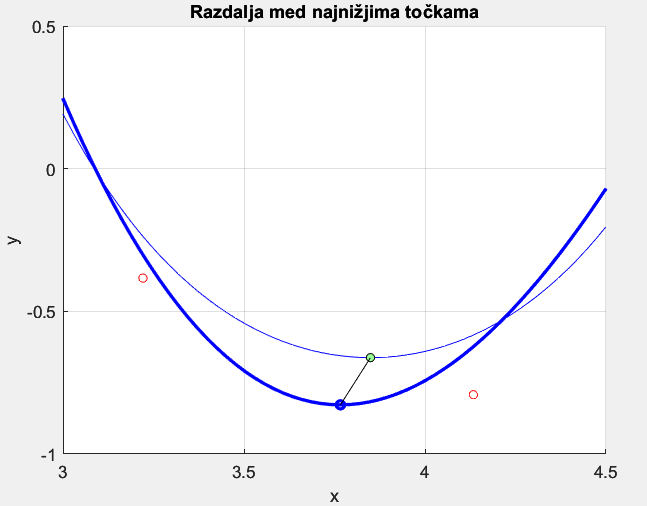
\includegraphics[width=0.8\linewidth]{razdalja.png}
            \caption{Razdalja}
            \label{fig:enter-label}
        \end{figure}

	\section{Viri in literatura}
        	
    	\begin{enumerate}[label=\textbullet]
    		\item Zapiski s predvanj in vaj pri predmetu Matematično modeliranje, dostopno: \href{https://ucilnica.fmf.uni-lj.si/course/view.php?id=135}{Spletna učilnica}
    		\item Teorija za izračun dolžine krivulje, dostopno na \href{https://mathinsight.org/length\_curves\_refresher}{Math Inside}.
    		\item Matlabov center za pomoč in dokumentacija vgrajenih funkcij \href{https://ch.mathworks.com/help/matlab/ref/polyfit.html}{Math Works}.
    		\item Matlab: Curve Fitting (polyfit and polyval) \href{https://www.youtube.com/watch?v=GOwPA1LPDaQ&t=374s}{Youtube}.
    	\end{enumerate}
 
\end{document}
